%نام و نام خانوادگی:
%شماره دانشجویی: 
\مسئله{پارسر LR(1)}


\پاسخ{

\begin{figure}[H]
			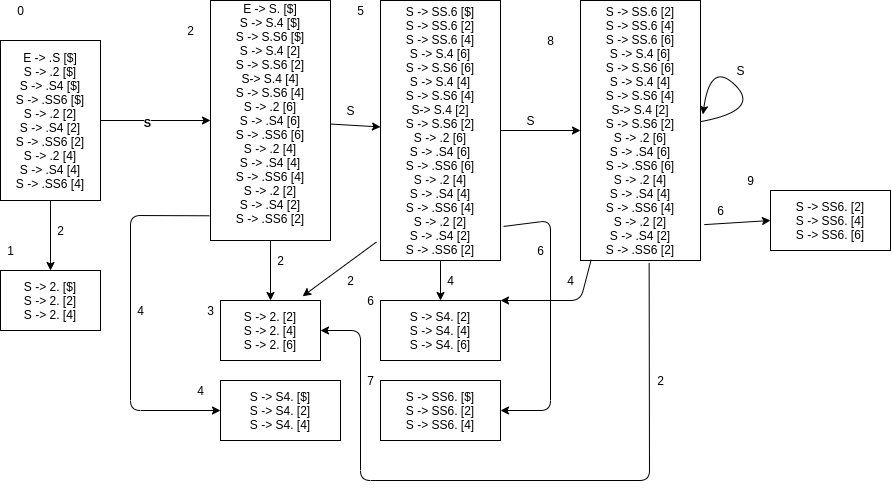
\includegraphics[width=\linewidth]{./commons/Q8.png}
			\label{fig:Q8}
		\end{figure}

		\begin{table}[H]
			\begin{tabular}{c|c|c|c|c|c|c|c|c|c|c}
				 & 2   & 4   & 6  & \&   & S \\
				\hline
				0 & S1 &      &     &  & G2 \\
				1 &R1 &R1 &  &R1 &\\
				2 & S3 &  S4    &      & acc & G5 \\
				3 &  R1    & R1 &  R1    &      &     \\
				4 & R2  & R2 &  &   R2   &     \\
				5 & S3 & S6 & S7 &  & G8 \\
				6 & R2 & R2 & R2 &  &  \\
				7 & R3 & R3 &  & R3 &  \\
				8 & S3 & S6 & S9 &  & G8 \\
				9 & R3 & R3 & R3 &  &  \\

				\hline
			\end{tabular}
		\end{table}
		
ابتدا در state شماره 0 هستیم. 2 را می‌بینیم و بهstate شماره 1 می‌رویم. سپس دوی بعدی را به عنوان lookahead انتخاب می‌کنیم. در s1 به ازای look a head 2 عمل reduce با قاعده تولید شماره یک را داریم.پس به 2 و s1 را خط می‌زنیم و S را جایگزین می‌کنیم. همین روند را تا آخر به صورت زیر ادامه می‌دهیم
\lr{
\\0 -> 2 -> S1 , look a head = 2
\\0 -> S -> G2 -> 2 -> S3 , look a head = 6
\\ 0 -> S -> G2 -> S -> G5 -> 6 -> S7 , look a head = 4
\\ 0 > S -> G2 -> 4 -> S4 , look ahead = 2
\\ 0 -> S -> G2 -> 2 -> S3 , look a head = 2
\\ 0 -> S -> G2 -> S -> G5 -> 2 -> S3 , look a head = 4
\\ 0 -> S -> G2 -> S -> G5 -> S -> G8 -> 4 -> S6 , look a head = 6
\\ 0 -> S -> G2 -> S -> G5 -> S -> G8 -> 6 - > S9 , look a head = 6
\\ 0 -> S -> G2 -> S -> G5 -> 6 -> S7  , look a head = \&
\\0 -> S ->G2 -> \& -> Accept \\
}


}